\documentclass[10pt,handout]{beamer}
%\documentclass[10pt]{beamer}
\usepackage[english]{babel} % Anpassa efter svenska. Ger svensk logga.
\usepackage[utf8]{inputenc} % Anpassa efter linux
\usepackage{graphicx}
\usepackage{hyperref}
\usepackage{listings}

\hypersetup{
    colorlinks=true,
    linkcolor=blue,
    filecolor=magenta,
    urlcolor=cyan,
}

\usetheme{Uppsala}
%\usecolortheme{UU} % Anpassa efter UU:s frger och logga
%\hypersetup{pdfpagemode=FullScreen} % Adobe Reader ska ppna fullskrm
\setbeamertemplate{itemize items}[circle]

% \usepackage{beamerthemesplit}
\usepackage{amsmath}
% \usepackage{amssymb}
% \usepackage{graphics}
% \usepackage{graphicx}
% \usepackage{epsfig}
% \usepackage[latin1]{inputenc}
 \usepackage{color}
% \usepackage{fancybox}
% \usepackage{psfrag}
% \usepackage[english]{babel}
 \setbeamertemplate{footline}{\hfill\insertframenumber/\inserttotalframenumber}

% Input new commands
%\usepackage{bm}
%\usepackage{natbib}
\newcommand{\bfm}[1]   {\mbox{\boldmath{${#1}$}}}
\newcommand{\Prob}   {\mbox{\textnormal{P}}}
\def\eqd{\,{\buildrel d \over =}\,}

% Vector/Matrix definitions (in bold type)
\newcommand{\vect}[1]{\mathbf{#1}}
\newcommand{\vectb}[1]{\bm{#1}}

% Differential operator 'd' as upright as in (use \dd)
\newcommand{\dd}{\; \mathrm{d}}

% Gaussian normal distribution (use \N)
\newcommand{\N}{\mathcal{N}} %% or \mathrm{N}

% Uniform distribution (use \Uni or \U)
\newcommand{\Uni}{\mathcal{U}} %% or \mathrm{U}
\newcommand{\U}{\mathcal{U}} %% or \mathrm{U}

% Matrix transpose (use \T)
\newcommand{\T}{^{\mathsf{T}}}

% Blockdiagonal matrices (use \blockdiag)
\newcommand{\blockdiag}{\mathrm{blockdiag}}

% Define inner product '<f,g>' notation (use \innerp{#1})
\providecommand{\innerp}[1]{\left\langle#1\right\rangle}

\def\o{{\mathbf o}}
\def\t{{\mathbf \theta}}
\def\w{{\mathbf w}}
\def\x{{\mathbf x}}
\def\y{{\mathbf y}}
\def\z{{\mathbf z}}



% Other math symbols and notation
\newcommand{\D}{^\mathsf{\dagger}}
\newcommand{\R}{\mathbb{R}}
\newcommand{\erf}{\mathrm{erf}}
\newcommand{\E}{\mathrm{E}}
\newcommand{\var}{\mathrm{var}}
\newcommand{\Var}{\mathrm{Var}}
\newcommand{\cov}{\mathrm{cov}}
\newcommand{\Ker}{\operatorname{Ker}}
\newcommand{\Ran}{\operatorname{Ran}}
\providecommand{\norm}[1]{\lVert#1\rVert}
\providecommand{\op}[1]{\mathcal{#1}}
\newcommand{\arccot}{\mathrm{arccot}}
\providecommand{\Hspace}[1]{\mathscr{#1}}
\providecommand{\fourier}[1]{\mathscr{#1}}

\newcommand{\kin}{k^{\rm in}}
\newcommand{\kout}{k^{\rm out}}
\newcommand{\gi}{{R_0}}
\newcommand{\eff}{{E_{\rm max}}}
\newcommand{\ESS}{\mathrm{ESS}}
\newcommand{\HN}{{\rm N^+}}
\newcommand{\lN}{{\rm LN}}

\DeclareMathOperator{\Sd}{Sd}
\DeclareMathOperator{\sd}{sd}
\DeclareMathOperator{\Gammad}{Gamma}
\DeclareMathOperator{\Invgamma}{Inv-gamma}
\DeclareMathOperator{\Bin}{Bin}
\DeclareMathOperator{\Negbin}{Neg-bin}
\DeclareMathOperator{\Poisson}{Poisson}
\DeclareMathOperator{\Beta}{Beta}
\DeclareMathOperator{\logit}{logit}
\DeclareMathOperator{\BF}{BF}
\DeclareMathOperator{\Invchi2}{Inv-\chi^2}
\DeclareMathOperator{\NInvchi2}{N-Inv-\chi^2}
\DeclareMathOperator{\InvWishart}{Inv-Wishart}
\DeclareMathOperator{\tr}{tr}
% \DeclareMathOperator{\Pr}{Pr}
\def\euro{{\footnotesize \EUR\, }}
\DeclareMathOperator{\rep}{\mathrm{rep}}


%%%%%%%%%%%%%%%%%%%%%%%%%%%%%%%%%%%%%%%%%%%%%%%%%%%%%%%%%%%%%%%%%%

\setlength{\parskip}{3mm}
\title[]{{\color{black}Bayesian Statistics and Data Analysis \\ Lecture 1}}
\author[]{M{\aa}ns Magnusson \\ Department of Statistics, Uppsala University}
\date{}

\begin{document}

\frame{\titlepage
% \thispagestyle{empty}
}

%%%%%%%%%%%%%%%%%%%%%%%%%%%%%%%%%%%%%%%%%%%%%%%%%%%%%%%%%%%%%%%%%%


\section{Introduction}
\frame{\sectionpage}

\begin{frame}

  \frametitle{Decision making in case of uncertainties}

  \begin{center}
    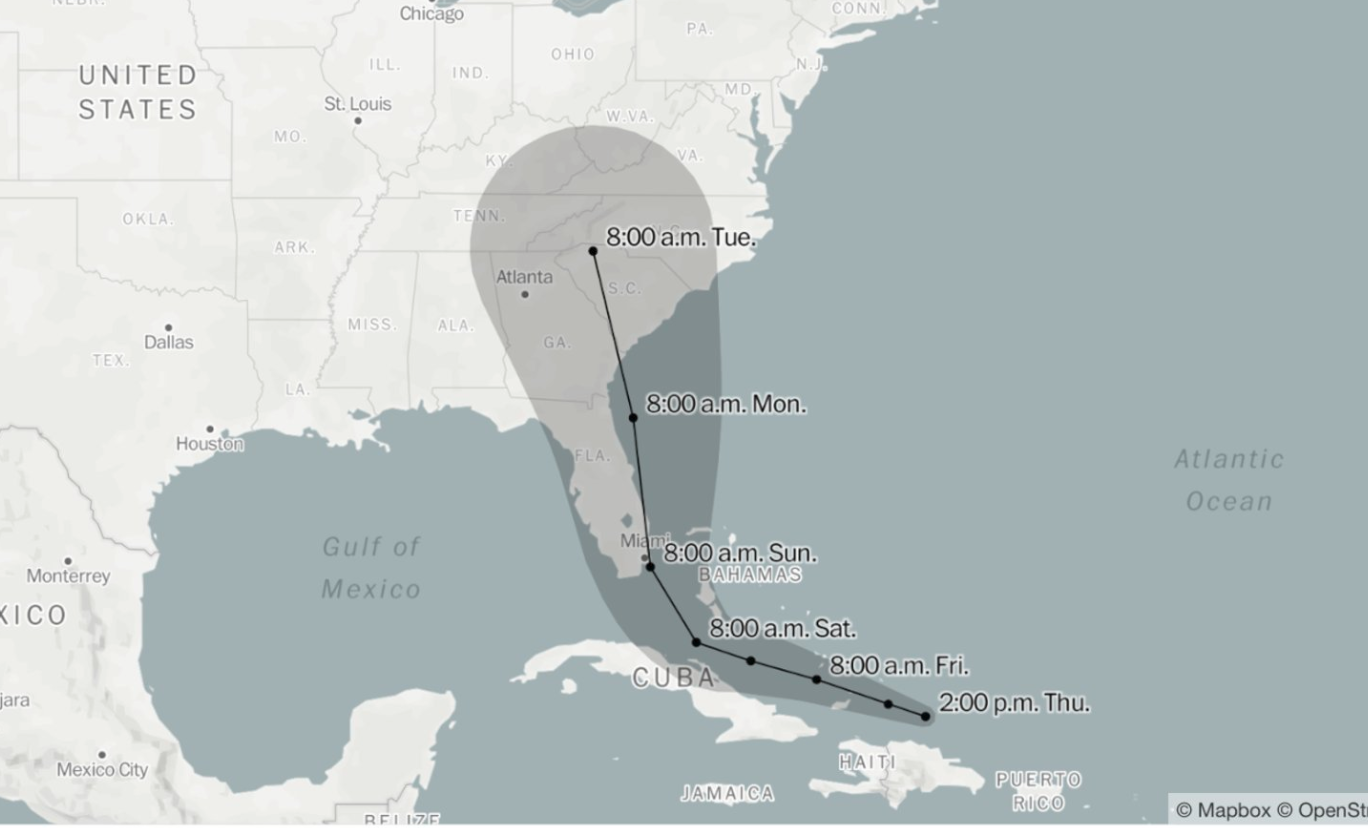
\includegraphics[width=10.5cm]{figs/irma.png}
  \end{center}
\end{frame}


\begin{frame}{Bayesian Analysis}

  \begin{itemize}
  \item Based on Bayesian probability theory
    \begin{itemize}
    \item uncertainty is presented with probabilities
    \item probabilities are updated based on new information
    % \item {\it ...common sense reduced to calculation},
    %   Laplace 1819
    \end{itemize}
    \pause
    \item Thomas Bayes (170?--1761)
    \begin{itemize}
    \item English nonconformist, Presbyterian minister,
      mathematician
    % \item Richard Price published Bayes' paper on conditional
    %   probabilities in 1763 after Bayes had died
    \item considered the problem of {\it inverse probability}
      \begin{itemize}
        \item significant part of the Bayesian theory
      \end{itemize}
  \end{itemize}
  \pause
  \item Bayes did not invent all, but was first to solve problem of
    inverse probability in special case
  \item Modern Bayesian theory with rigorous proofs developed in
    20th century
\end{itemize}
\end{frame}

\begin{frame}{Term Bayesian used first time in mid 20th century}

  \begin{itemize}
  \item Earlier there was just "probability theory"
    \begin{itemize}
    \item concept of the probability was not strictly defined,
      although it was close to modern Bayesian interpretation
    \item in the end of 19th century there were increasing demand
      for more strict definition of probability (mathematical and
      philosophical problem)
    \end{itemize}
    \pause
    \item In the beginning of 20th century frequentist view gained popularity
    \begin{itemize}
    \item accepts definition of probabilities only through frequencies
    \item does not accept inverse probability or use of prior
    \item gained popularity due to apparent objectivity and "cook
      book" like reference books
    \end{itemize}
    \pause
    \item R. A. Fisher used in 1950 first
      time term "Bayesian" to emphasize the difference to general
      term "probability theory"
      \begin{itemize}
      \item term became quickly popular, because alternative
        descriptions were longer
    %     \pause
    % \item after this Bayesians started to use term "frequentist"
    \end{itemize}
\end{itemize}
\end{frame}

\begin{frame}{Uncertainty and probabilistic modeling}

  \begin{itemize}
  \item Two types of uncertainty: aleatoric and epistemic
    \vspace{\baselineskip}
  \item Representing uncertainty with probabilities
    \vspace{\baselineskip}
  \item Updating uncertainty
   \end{itemize}
\end{frame}


\begin{frame}{Two types of uncertainty}

  \begin{itemize}
  \item Aleatoric uncertainty due to randomness
    \begin{itemize}
    \item<2-> we are not able to obtain observations which could reduce
      this uncertainty
    \end{itemize}
    \vspace{\baselineskip}
  \item Epistemic uncertainty due to lack of knowledge
    \begin{itemize}
    \item<3-> we are able to obtain observations which can reduce
      this uncertainty
    \item<3-> two observers may have different epistemic uncertainty
    %\item<3-> epistemic uncertainty chances when the information chances
    \end{itemize}
  \end{itemize}
\end{frame}


\begin{frame}{Updating uncertainty}

  \begin{itemize}
  %\item<2-> probability of red $\frac{\mathrm{\#red}}{\mathrm{\#red+\#yellow}}{\onslide<3->=\theta}$
  \item<2-> Probability of red $\frac{\mathrm{\#red}}{\mathrm{\#red+\#yellow}}=\theta$
    \vspace{\baselineskip}
  \item<3-> $p(y=\mathrm{red}|\theta)=\theta \quad$ aleatoric uncertainty
    \vspace{\baselineskip}
  \item<4-> $p(\theta) \quad$ epistemic uncertainty
    \vspace{\baselineskip}
  \item<5-> Picking many chips updates our uncertainty about the proportion
    \vspace{\baselineskip}
  \item<5-> $p(\theta|\mathrm{y=red,yellow,red,red,\ldots})=?$
    \vspace{\baselineskip}
  \item<6-> Bayes rule
      $p(\theta|y)=\frac{p(y|\theta)p(\theta)}{\int p(y|\theta)p(\theta) d\theta}$
  \end{itemize}
\end{frame}


\begin{frame}{Model vs. likelihood}

  \begin{itemize}
  \item Bayes rule
      $p(\theta|y)\propto p(y|\theta)p(\theta)$
    \vspace{\baselineskip}
  \item Model: $p(y|\theta)$ as a function of $y$ given fixed $\theta$
    describes the aleatoric uncertainty \vspace{\baselineskip}
  \item Likelihood: $p(y|\theta)$ %=L(\theta|y)$
    as a function of $\theta$
    given fixed $y$ provides information about epistemic uncertainty,
    but is not a probability distribution
    \vspace{\baselineskip}
  \item<2-> Bayes rule combines the likelihood with prior uncertainty
    $p(\theta)$ and transforms them to updated posterior uncertainty
  \end{itemize}
\end{frame}

%% TODO: Change example

\begin{frame}{Example application: Drug dosage for liver transplant\footnote{\color{gray}with E. Siivola, Aalto and S. Weber, Novartis Pharma}}

  \vspace{-0.5\baselineskip}
\begin{itemize}
\item Everolimus is immunosuppressant to prevent rejection of organ
  transplants
\item Pharmacokinetic model of drug and body, optimal dosage depends on weight\\
  \begin{minipage}[t]{\textwidth}
    \vspace{-.2\baselineskip}
  \hspace{-1.2cm}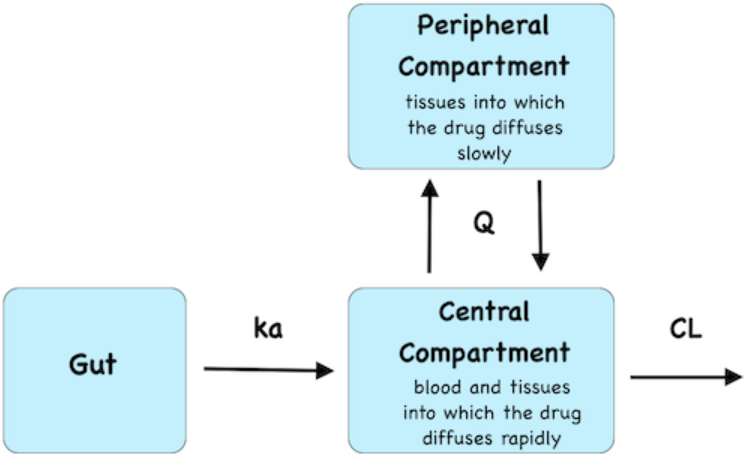
\includegraphics[width=6cm]{figs/2compartment_graph.png}
  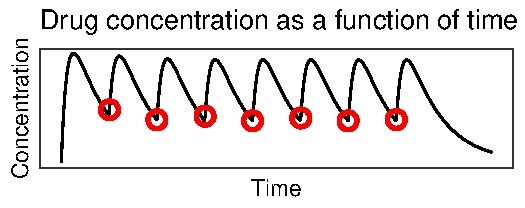
\includegraphics[width=6cm]{figs/data_population_simple.pdf}
\end{minipage}
    \vspace{.2\baselineskip}
\item<2-> Model fitted with 500 adults, extrapolation to children?
\item<3-> Maturation effect, 17 observations from children
\end{itemize}

\end{frame}

\begin{frame}{The art of probabilistic modeling}

  \begin{itemize}
  \item The art of probabilistic modeling is to describe in a
    mathematical form (model and prior distributions) what we already
    know and what we don't know
\vspace{\baselineskip}
  \item<2-> ``Easy'' part is to use Bayes rule to update the uncertainties
    \begin{itemize}
    \item computational challenges
    \end{itemize}
\vspace{\baselineskip}
  \item<3-> Other parts of the art of probabilistic modeling are, for example,
    \begin{itemize}
    \item model checking: is data in conflict with our prior knowledge?
    \item presentation: presenting the model and the results to the application experts
    \end{itemize}
  \end{itemize}
\end{frame}

\begin{frame}

  \begin{columns}[T] % align columns
 \begin{column}{.49\textwidth}
{  \footnotesize
  \begin{itemize}
 \item Galaxy clusters for cosmology
 \item Coagulation of blood
 \item Gene regulation
 \item Pharmacokinetics and -dynamics
 \item Decision support
 \item Effects of nutrition for diabetes
 \item Evolutionary anthropology
 \item Clinical trial designs
 \item Daily demand for gas
 \item Brain structure trees
 \item School enrollment
 \item Sports
 \item Product demand
 \end{itemize}
 }
\end{column}
 \begin{column}{.49\textwidth}
{    \footnotesize
  \begin{itemize}
 \item Cocoa bean fermentation
 \item Marine propulsion power
 \item Alcohol consumption trends
 \item Flood probability
 \item Instantaneous heart rate distributions
 \item Drug dosing regimens in pediatrics
 \item Human T stem cell memory cells
 \item Fairness in university admission policies
 \item Destruction of bacteria and bacterial spores under heat
 \end{itemize}
 }
\end{column}
\end{columns}
\end{frame}

\begin{frame}
  \frametitle{Bayesian data analysis}  %
  \framesubtitle{Example analyses}
  \begin{itemize}
  \item Treatment/control
    \begin{itemize}
    \item randomize patients to treatment or control
    \item is the treatment effective?
    \end{itemize}
    \pause
  \item Continuous valued treatment
    \begin{itemize}
    \item randomize patients with different dosages
    \item which dosage is sufficient without too many side effects?
    \end{itemize}
    \pause
  \item Different effects for different patients?
    \begin{itemize}
    \item Is the treatment effect different for male/female, child/adult, light/heavy, ...
    \end{itemize}
  \end{itemize}

\end{frame}

\begin{frame}{Bayesian approach}

  \begin{itemize}
  \item Benefits of Bayesian approach
    \begin{itemize}
    \item integrate over uncertainties to focus to interesting parts
    \item use relevant prior information
    \item hierarchical models
    \item model checking and evaluation
    \end{itemize}
  \end{itemize}
\end{frame}

\begin{frame}{Computation}

  We need to be able to compute expectations with respect to posterior
  distribution $p(\theta|y)$
  \begin{align*}
    \E_{\theta|y}\left[ g(\theta) \right] = \int p(\theta|y)g(\theta) d\theta
  \end{align*}

  \begin{itemize}
  \item Analytic
    \begin{itemize}
    \item only for very simple models
    \end{itemize}
  \item Monte Carlo, Markov chain Monte Carlo
    \begin{itemize}
    \item generic
    \end{itemize}
  \item Distributional approximations
    \begin{itemize}
    \item e.g. Laplace, variational, expectation propagation
    \item less generic, but can be much faster with sufficient accuracy
    \end{itemize}
  \end{itemize}
\end{frame}

\begin{frame}

  \frametitle{Probabilistic programming}

  \begin{center}
   \vspace{-\baselineskip}
    
\includegraphics[width=5cm]{figs/wide_ensemble.png}\\
   \vspace{2\baselineskip}
  {\large Enables agile workflow for developing probabilistic models}\\
   \vspace{\baselineskip}
   language \, -- \,
   automated inference \, -- \,
   diagnostics
   \vspace{\baselineskip}
  \vfill
    
\includegraphics[width=1.5cm]{figs/stan_logo_wide.png}\\
    \url{mc-stan.org}
  \end{center}

\end{frame}

\begin{frame}[fragile]
  \frametitle{Binomial model for treatment/control comparison}

  \begin{itemize}
  \item Two groups of patients: treatment and control
    \begin{itemize}
    \item Binary outcome
    \item Is the treatment useful?
    \end{itemize}
  \end{itemize}

\end{frame}

\begin{frame}[fragile]
  \frametitle{Binomial model for treatment/control comparison}
  {\footnotesize
  \begin{lstlisting}
data {
  int<lower=0> N1;
  int<lower=0> y1;
  int<lower=0> N2;
  int<lower=0> y2;
}
parameters {
  real<lower=0,upper=1> theta1;
  real<lower=0,upper=1> theta2;
}
model {
  theta1 ~ beta(1,1);
  theta2 ~ beta(1,1);
  y1 ~ binomial(N1,theta1);
  y2 ~ binomial(N2,theta2);
}
generated quantities {
  real oddsratio;
  oddsratio = (theta2/(1-theta2))/(theta1/(1-theta1));
}
  \end{lstlisting}
}
\end{frame}

\begin{frame}[fragile]
  \frametitle{Binomial model for treatment/control comparison}

  RStanARM
  {\scriptsize
  \begin{lstlisting}
    fit_bin2 <- stan_glm(y/N ~ grp2, family = binomial(),
                         data = d_bin2, weights = N)
  \end{lstlisting}
}
\end{frame}

\begin{frame}{Modeling nature}

  \begin{itemize}
  \item Drop a ball from different heights and measure time
    \pause
    \begin{itemize}
    \item Newton
    \item air resistance, air pressure, shape and surface structure of the ball
    \item relativity
    \end{itemize}
    \pause
  \item Taking into account the accuracy of the measurements, how
    accurate model is needed?
    \pause
    \begin{itemize}
    \item often simple models are adequate and useful
    \item \emph{All models are wrong, but some of them are useful},
      George P. Box
    \end{itemize}
  \end{itemize}

\end{frame}

\begin{frame}{Reminder: Uncertainty and probabilistic modeling}

  \begin{itemize}
  \item Two types of uncertainty: aleatoric and epistemic
    \vspace{\baselineskip}
  \item Representing uncertainty with probabilities
    \vspace{\baselineskip}
  \item Updating uncertainty
    \vspace{\baselineskip}
  %   \pause
  % \item Additional reading material in Noppa (see Lecture 1)
   \end{itemize}
\end{frame}

\begin{frame}{Questions}

  \begin{itemize}
  \item<1-> Pick a number between 1--5
    \begin{itemize}
    \item<2-> raise as many fingers
    \item<3-> is the number of fingers raised random (by you or by others)?
    \end{itemize}
    \vspace{\baselineskip}
  \item<4-> If we build a robot with very fast vision which can observe
    the rotating coin accurately, is the throw random for the robot?
    \vspace{\baselineskip}
  \item<5-> Is the quantum uncertainty aleatoric or epistemic?
    \vspace{\baselineskip}
  \item<6-> What is your own example with both aleatoric and epistemic
    uncertainty?
  \end{itemize}
\end{frame}

\begin{frame}{Rest of the course}

  \begin{itemize}
  \item Basic models which can be used as building blocks
    \vspace{\baselineskip}
  \item Basic computation
    \vspace{\baselineskip}
  \item Typical simple scientific data analysis cases
     \begin{itemize}
     \item e.g. comparison of treatments
     \end{itemize}
    \vspace{\baselineskip}
  \item Presentation of the results
  \end{itemize}
\end{frame}

\begin{frame}{Some important terms}

  \begin{itemize}
  \item[-] probability
  \item[-] probability density
  \item[-] probability mass
  \item[-] probability density function (pdf)
  \item[-] probability mass function (pmf)
  \item[-] probability distribution
  \item[-] discrete probability distribution
  \item[-] continuous probability distribution
  \item[-] cumulative distribution function (cdf)
  \item[-] likelihood
  \end{itemize}

\end{frame}

\begin{frame}{Ambiguous notation in statistics}

  \begin{itemize}
  \item[] In $p(y|\theta)$
    \pause
  \begin{itemize}
  \item[-] $y$ can be variable or value
    \begin{itemize}
    \item[] we could clarify by using $p(Y|\theta)$ or $p(y|\theta)$
    \end{itemize}
    \pause
  \item[-] $\theta$ can be variable or value
    \begin{itemize}
    \item[] we could clarify by using $p(y|\Theta)$ or $p(y|\theta)$
    \end{itemize}
    \pause
  \item[-] $p$ can be a discrete or continuous function of $y$ or $\theta$
    \begin{itemize}
    \item[] we could clarify by using $P_Y$, $P_\Theta$, $p_Y$ or $p_\Theta$
    \end{itemize}
    \pause
\item[-]
  $P_Y(Y|\Theta=\theta)$ is a probability mass function, sampling distribution, observation model
    \pause
\item[-]
$P(Y=y|\Theta=\theta)$ is a probability
    \pause
\item[-]
$P_\Theta(Y=y|\Theta)$ is a likelihood function (can be discrete or continuous)
    \pause
\item[-] $p_Y(Y|\Theta=\theta)$ is a probability density function, sampling distrbution, observation model
    \pause
\item[-] $p(Y=y|\Theta=\theta)$ is a density
    \pause
\item[-] $p_\Theta(Y=y|\Theta)$ is a likelihood function (can be discrete or continuous)
    \pause
  \item[-] $y$ and $\theta$ can also be mix of continuous and discrete
    \pause
    \item[-] Due to the sloppines sometimes likelihood is used to refer
$P_{Y,\theta}(Y|\Theta)$, $p_{Y,\theta}(Y|\Theta)$

  \end{itemize}
\end{itemize}
\end{frame}



\end{document}



%%%%%%%%%%%%%%%%%%%%%%%%%%%%%%%%%%%%%%%%%%%%%%%%%%%%%%%%%%%%%%%%%%


\end{document}
